\documentclass[11pt,a4paper]{article}

\usepackage[margin=2.2cm]{geometry}
\usepackage[T1]{fontenc}
\usepackage{lmodern}
\usepackage{microtype}
\usepackage{amsmath}
\usepackage{xcolor}
\usepackage{booktabs}
\usepackage{tabularx}
\usepackage{array}
\usepackage{enumitem}
\usepackage{caption}
\usepackage{float}
\usepackage{titlesec}
\usepackage{tikz}
\usetikzlibrary{arrows.meta,positioning,fit,backgrounds,calc}
\usepackage[hidelinks]{hyperref}

\definecolor{accent}{HTML}{0E6B5C}
\definecolor{soft}{HTML}{E4F1EE}
\definecolor{warn}{HTML}{B4492C}
\definecolor{muted}{HTML}{56635E}

\titleformat{\section}{\large\bfseries\color{accent}}{\thesection}{0.6em}{}
\titleformat{\subsection}{\normalsize\bfseries}{\thesubsection}{0.5em}{}
\titlespacing*{\section}{0pt}{1.1em}{0.4em}
\titlespacing*{\subsection}{0pt}{0.8em}{0.3em}
\setlist{itemsep=1pt,topsep=3pt,leftmargin=1.4em}
\captionsetup{font=small,labelfont=bf}
\newcolumntype{L}{>{\raggedright\arraybackslash}X}
\newcolumntype{P}[1]{>{\raggedright\arraybackslash\hyphenpenalty=10000}p{#1}}
\renewcommand{\arraystretch}{1.15}
\setlength{\emergencystretch}{3em}

\newcommand{\rqlabel}[1]{\textbf{\color{accent}#1}}

\begin{document}

%-------------------------------------------------------------------- title
\begin{center}
  {\LARGE\bfseries Requirements as the Oracle:}\\[3pt]
  {\Large Generating REST API Tests from Vague Requirements\\ Without Learning the Bugs They Should Catch}\\[10pt]
  {\large\bfseries Team PreTrained}\\[4pt]
  {\small\begin{tabular}{@{}l@{\hspace{1.2em}}l@{\hspace{3em}}l@{\hspace{1.2em}}l@{}}
Sohail Memon & 2025201075 & Mohd Ahmad & 2025201029\\
Kathan Patel & 2025201039 & Md Taufique Hussain & 2025202007
\end{tabular}}
\end{center}

%-------------------------------------------------------------------- 1
\section{Domain and Target User}
\textbf{Domain:} Software engineering, specifically functional testing of REST (web) APIs.\\
\textbf{Target users:} Backend developers and QA engineers who have natural-language requirements (user stories, acceptance criteria) and an OpenAPI specification, and want automated tests that check the API \emph{behaves} as required, not only that it does not crash.

%-------------------------------------------------------------------- 2
\section{Problem Statement}
Automated REST API testing tools are effective at finding crashes. AutoRestTest won the SBFT~2026 REST tool competition, detecting about 2.7$\times$ more faults than the next tool~\cite{sbft26,autoresttest}. However, these tools use HTTP~5xx responses as their oracle, so a requirement violation that returns \texttt{200 OK} (e.g.\ a user deleting another user's data) goes undetected. Catching such bugs requires knowing the \emph{expected} behaviour, which lives in natural-language requirements. RESTestBench~\cite{restestbench} measured how well LLMs turn requirements into executable tests: the best model catches up to 92\% of planted bugs with precise requirements, but only 2--54\% with vague ones, which is the realistic case in practice. A refinement loop (run the test, read the HTTP trace, regenerate) improves results, yet when the service under test is faulty the model ``adapts its assertions to match the faulty behaviour''~\cite{restestbench}, so the refined test encodes the bug as correct. The paper measures this effect but proposes no remedy. Our problem is therefore to generate effective tests from vague requirements \emph{and} to make refinement safe on possibly-buggy services.

%-------------------------------------------------------------------- 3
\section{Research Questions and Hypotheses}
\begin{description}[leftmargin=0pt,labelsep=0.4em]
\item[\rqlabel{RQ1 (vague requirements).}] Given only a vague requirement and the OpenAPI specification, with no human input and no precise version at test time, can an LLM agent generate tests that catch requirement-violating bugs? How much of the vague-to-precise gap can it close?
\item[\rqlabel{RQ2 (safe refinement).}] Does restricting refinement (locked checks, hidden observed values on assertion failures, strengthen-only edits, an evidence-restricted judge) remove bug adaptation \emph{without} increasing false alarms on the correct service?
\item[\rqlabel{RQ3 (component value).}] Which components (requirement-precision layer, retrieval, tool-based execution, restricted refinement, judge, fine-tuning) contribute measurably, and which variant of each works best? Can a fine-tuned 8B model approach a cheap API model?
\end{description}
\textbf{Hypotheses.} \textbf{H1:} deriving implied properties (round-trip, echo, ownership, before/after deltas, filter correctness) raises the bug-catching score on vague requirements well above the single-step baseline. \textbf{H2:} with restricted refinement, the score of tests refined against the buggy service is close to that of tests refined against the correct service (adaptation gap $\approx 0$), with a false-alarm rate no higher than unrestricted refinement. \textbf{H3:} tool-based execution sharply reduces tests that fail on the correct service, which is the dominant failure of small models.

%-------------------------------------------------------------------- 4
\section{Why the Problem Matters}
\begin{itemize}
  \item Real requirements are vague. A test generator that works only on carefully written specifications has limited practical value.
  \item A test that silently accepts a bug is worse than no test, because it gives false confidence. Teams increasingly let LLMs write tests, so this failure mode will reach production code.
  \item Small models are cheap enough to run on every commit, but our re-analysis (Section~\ref{sec:prelim}) shows they currently fail on both problems.
\end{itemize}

%-------------------------------------------------------------------- 5
\section{What Is Missing in Existing Approaches}
\begin{table}[H]
\centering\small
\begin{tabularx}{\linewidth}{@{}P{3.6cm}LL@{}}
\toprule
\textbf{Approach} & \textbf{Reported performance} & \textbf{Gap for our problem}\\
\midrule
Crash-oriented fuzzers: EvoMaster, RESTler, AutoRestTest~\cite{autoresttest}, LlamaRestTest~\cite{llamaresttest}, APIPilot~\cite{apipilot} & AutoRestTest: 58.3\% method coverage, 42 server errors on 12 services; SBFT~2026 winner & Oracle is 5xx/schema only; requirement violations returning 200 are invisible\\
Response-judging agents: LogiAgent~\cite{logiagent}, ARMeta~\cite{armeta} & LogiAgent: 234 logical issues, 66.2\% accuracy; ARMeta: 57--79\% true-positive rate & Judge sees the response before deciding, so it shares the same bias; many false alarms\\
Oracle generation: SATORI~\cite{satori}, MASTOR~\cite{mastor} & SATORI F1 74.3\% (spec only); MASTOR 75.4\% mutation score (needs Java source) & No requirements; MASTOR derives ``truth'' from the implementation\\
Requirement-based generation: APITestGenie~\cite{apitestgenie}, RESTestBench baselines~\cite{restestbench} & APITestGenie: 69.3\% valid scripts on 25 requirements; RESTestBench: 2--54\% on vague requirements & Refinement freely rewrites expectations, so tests learn bugs; no remedy proposed\\
\bottomrule
\end{tabularx}
\caption{State of the art (numbers as reported by each paper on its own setup; not directly comparable).}
\end{table}

\noindent LLM-generated test oracles are known to capture the \emph{actual} rather than the \emph{expected} program behaviour~\cite{konstantinou}, which is the mechanism behind bug adaptation.

\subsection{Preliminary analysis of RESTestBench's released code and results}\label{sec:prelim}
We inspected the authors' prompts and raw result files. Two findings motivate our design:
\begin{enumerate}
  \item \textbf{The refinement prompts encourage adaptation.} The judge's few-shot example marks ``the test expects \texttt{'Authentication failed'}, but the actual response contains \texttt{'Authentication error'}'' as needing refinement, i.e.\ it teaches copying the observed value. The generator is told to ``use the Test Execution Output and the HTTP Trace to enhance the test'' and is never warned the service may be buggy. The judge's reasoning is not passed on (\texttt{USE\_JUDGE\_FEEDBACK\_IN\_REFINEMENT = False}), and there is no ``API bug'' outcome.
  \item \textbf{Small models fail on mechanics and adapt to bugs.} For Llama~3.1~8B, excluding a failed run (0 valid tests), the share of planted bugs caught on vague requirements is 3.1\% single-step, 12.3\% after refinement on the correct service, and 3.5\% after refinement on the buggy service: the entire refinement gain disappears. Across settings, 44--100\% of its tests fail even on the correct service. (The paper's 13\% figure for this model appears to include the failed run; without it, precise single-step is about 20\%.)
\end{enumerate}

%-------------------------------------------------------------------- 6
\section{Capabilities Used and Why the Problem Needs Each}
\begin{table}[H]
\centering\small
\begin{tabularx}{\linewidth}{@{}P{2.3cm}LL@{}}
\toprule
\textbf{Capability} & \textbf{Why the problem needs it} & \textbf{How we measure it}\\
\midrule
Tool calling & Small models get login flows, URLs, payloads and ID passing wrong; these are exact operations that tools can do deterministically from the spec & Valid-request rate, setup-error rate, tool-call argument validity, recovery after errors\\
Agentic & Testing is multi-step: create data, chain calls, observe state, decide whether a failure is the API's or the test's fault, and stop & Requirements completed end-to-end, steps per requirement, abstention precision\\
RAG & Specs are large; pasting the full spec (as RESTestBench does) overloads small models and wastes tokens & Recall@k, MRR, nDCG of retrieved operations; context tokens\\
Reasoning & Vague requirements must be expanded into concrete checks; the judge must reason about blame from evidence & Check recall and contradiction rate vs.\ precise requirements; judge verdict accuracy\\
Fine-tuning & Cost and the adaptation bias itself: train a small model to derive checks (SFT) and to report bugs instead of copying (DPO) & Bug-catching score, adaptation gap and cost vs.\ base 8B and an API model\\
\bottomrule
\end{tabularx}
\caption{The five capabilities, the reason each is needed, and its metric.}
\end{table}

%-------------------------------------------------------------------- 7
\section{Proposed Approach and Architecture}

\begin{figure}[h]
\centering
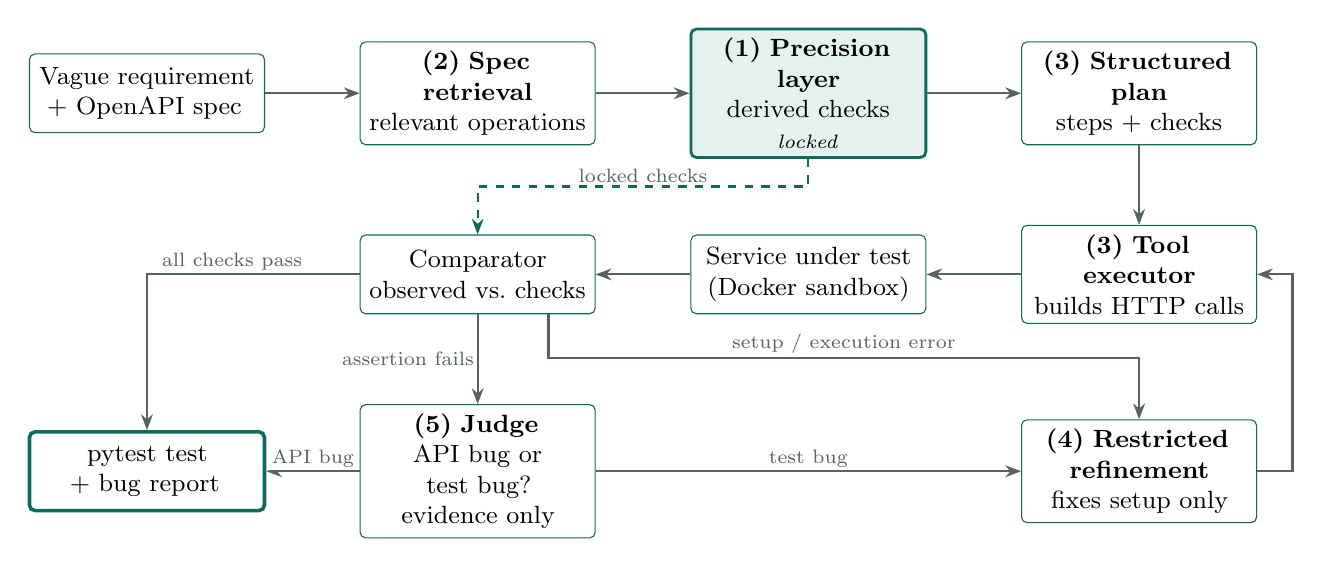
\begin{tikzpicture}[
  box/.style={draw=accent,fill=white,rounded corners=2pt,align=center,font=\small,minimum height=10mm,text width=2.75cm,execute at begin node={\hyphenpenalty=10000}},
  lock/.style={box,fill=soft,line width=1pt},
  outb/.style={box,line width=1.3pt},
  arr/.style={-{Stealth[length=2mm]},thick,color=muted},
  lab/.style={font=\scriptsize,color=muted,fill=white,inner sep=1pt}]
\node[box]  (req)   at (0,0)      {Vague requirement\\+ OpenAPI spec};
\node[box]  (rag)   at (4.2,0)    {\textbf{(2) Spec retrieval}\\relevant operations};
\node[lock] (prec)  at (8.4,0)    {\textbf{(1) Precision layer}\\derived checks\\{\scriptsize\itshape locked}};
\node[box]  (plan)  at (12.6,0)   {\textbf{(3) Structured plan}\\steps + checks};
\node[box]  (exec)  at (12.6,-2.3) {\textbf{(3) Tool executor}\\builds HTTP calls};
\node[box]  (sut)   at (8.4,-2.3)  {Service under test\\(Docker sandbox)};
\node[box]  (cmp)   at (4.2,-2.3)  {Comparator\\observed vs.\ checks};
\node[box]  (judge) at (4.2,-4.8)  {\textbf{(5) Judge}\\API bug or test bug?\\evidence only};
\node[outb] (out)   at (0,-4.8)    {pytest test\\+ bug report};
\node[box]  (ref)   at (12.6,-4.8) {\textbf{(4) Restricted refinement}\\fixes setup only};
\draw[arr] (req) -- (rag);
\draw[arr] (rag) -- (prec);
\draw[arr] (prec) -- (plan);
\draw[arr] (plan) -- (exec);
\draw[arr] (exec) -- (sut);
\draw[arr] (sut) -- (cmp);
\draw[arr,dashed,color=accent] (prec.south) -- ++(0,-0.35) -| node[lab,pos=0.25,above]{locked checks} (cmp.north);
\draw[arr] (cmp) -- node[lab,left]{assertion fails} (judge);
\draw[arr] (cmp.west) -| node[lab,pos=0.3,above]{all checks pass} (out.north);
\draw[arr] (judge) -- node[lab,above]{API bug} (out);
\draw[arr] (judge) -- node[lab,above]{test bug} (ref);
\draw[arr] ($(cmp.south)+(0.9,0)$) -- ++(0,-0.55) -| node[lab,pos=0.25,above]{setup / execution error} (ref.north);
\draw[arr] (ref.east) -- ++(0.45,0) |- (exec.east);
\end{tikzpicture}
\caption{Proposed pipeline. Numbers refer to the components in the text. The shaded component is locked: execution feedback can fix how a test runs, but never the derived checks it compares against.}
\end{figure}

\begin{enumerate}[label=(\arabic*)]
\item \textbf{Requirement-precision layer.} Before any execution, the LLM expands the vague requirement into a set of atomic checks, guided by a small catalogue of implied properties (round-trip, echo, ownership/isolation, before/after deltas, filter soundness and completeness). Each check is tagged \emph{meaning} (business rule, locked) or \emph{format} (field names, envelopes, status codes the requirement does not fix; changeable only with spec evidence). The benchmark's precise requirements are used \emph{only for evaluation}, never as input.
\item \textbf{Spec retrieval (RAG).} Each OpenAPI operation (path, method, resolved schemas, description) is one chunk; the retriever returns the operations the requirement needs.
\item \textbf{Structured plan and tool executor.} The LLM outputs a plan (actors, setup, action, checks), not raw code. Deterministic tools build requests from the spec (authentication flow, URLs, required fields, ID passing) and compile the plan to a pytest test.
\item \textbf{Restricted refinement.} Execution errors (401/422 on setup, exceptions, missing spec-declared fields) are shown in full and may be fixed. Assertion failures are reported \emph{without the observed value}. A guard allows only strengthening edits and flags any new expected value equal to a value from the last response (value copying).
\item \textbf{Evidence-restricted judge.} On an assertion failure, the judge decides \textsc{API\_BUG} or \textsc{TEST\_BUG}, citing only requirement or spec text; ``the server returned it'' is never valid evidence. \textsc{API\_BUG} ends the loop and keeps the test. Uncertain cases abstain.
\item \textbf{Fine-tuning.} An 8B model (Llama~3.1~8B Instruct, for comparability with RESTestBench) trained with QLoRA: SFT on derived-check plans verified to catch planted bugs, then DPO preferring ``report bug'' over ``adapt to the response''. Leave-one-service-out training prevents leakage.
\end{enumerate}

%-------------------------------------------------------------------- 8
\section{Expected Novelty}
\begin{itemize}
  \item The first remedy for the bug-adaptation effect identified by RESTestBench, with a mechanism-level explanation (prompt analysis and value-copy measurement).
  \item Separation of a test's \emph{meaning} from its \emph{format}, with explicit evidence rules for when each may change.
  \item Requirement-free-at-test-time expansion of vague requirements into implied, verifiable properties, evaluated against the benchmark's precise requirements.
  \item A component-by-component study (variants and metrics per component) of an agentic API test generator, including preference fine-tuning against adaptation.
\end{itemize}

%-------------------------------------------------------------------- 9
\section{Dataset and Evaluation Environment}
\begin{itemize}
  \item \textbf{RESTestBench}~\cite{restestbench} (public): 3 Dockerised services (FastAPI/Python, NestJS RealWorld/TypeScript, TodoApp/.NET); 106 requirements (63/29/14), each in a vague and a precise version; 228 hand-written, requirement-specific mutants (141/65/22); one reference test per requirement; scoring harness.
  \item \textbf{Optional extension:} 2--3 further APIs from EMB/WFD or RESTgym with $\sim$40 requirements and $\sim$80 mutants in RESTestBench's format, to test generalisation.
  \item \textbf{Sandbox:} all services run locally in Docker; tools may only call the service's base URL.
\end{itemize}

%-------------------------------------------------------------------- 10
\section{Baselines}
All comparisons use the same LLM and budget.
\begin{enumerate}[label=B\arabic*.]
  \item RESTestBench single-step generation (their prompt).
  \item RESTestBench refinement loop (their prompts, 3 rounds).
  \item \emph{Prompt-fixed} refinement: their pipeline with only the prompts corrected (copying example removed, generator warned, judge feedback passed on, \textsc{API\_BUG} outcome). This isolates ``better prompting'' from our structural changes.
  \item A response-judging agent in the style of LogiAgent~\cite{logiagent}.
  \item A crash/schema fuzzer (EvoMaster or Schemathesis), to show which requirement bugs crash oracles miss.
\end{enumerate}
Reference points: published RESTestBench results for all 10 models, recomputed from the raw files with failed runs excluded.

%-------------------------------------------------------------------- 11
\section{Evaluation Plan and Metrics}
\subsection{End-to-end and safety metrics}
\begin{itemize}
  \item \textbf{Bug-catching score} (RESTestBench mutation score: mutants killed by tests that pass on the correct service), reported separately for vague and precise.
  \item \textbf{Gap closed} on vague requirements: $(\text{ours} - \text{baseline}) / (\text{precise upper bound} - \text{baseline})$.
  \item \textbf{Adaptation gap}: score of tests refined on the correct service minus score of tests refined on the buggy service.
  \item \textbf{False-alarm rate}: tests failing on the correct service.
  \item \textbf{Safety / unapproved actions:} expectation \emph{tampering rate} (value copying and weakening edits), calls outside the sandbox allow-list, forbidden test edits (\texttt{pytest.skip}, removed assertions). Target: zero accepted.
  \item \textbf{Tool-call accuracy}: correct tool, valid arguments, successful recovery.
  \item \textbf{Cost}: tokens, \$ and wall-clock time per requirement.
\end{itemize}

\subsection{Component-level evaluation (variants $\times$ metric)}
Following TA feedback, each component is justified by its own metric and compared across several variants.
\begin{table}[H]
\centering\small
\begin{tabularx}{\linewidth}{@{}P{2.6cm}LL@{}}
\toprule
\textbf{Component} & \textbf{Variants} & \textbf{Component metric (ground truth)}\\
\midrule
Precision layer & none; direct rewrite; property-catalogue guided; self-consistency (5 drafts, majority); fine-tuned 8B & Check recall, contradiction rate, invented-check rate (atomic checks of the precise requirement)\\
Retrieval & full spec (no RAG); BM25; dense; hybrid (BM25+dense, RRF); hybrid + cross-encoder reranker; + LLM query rewriting & Recall@k, MRR, nDCG, context tokens (operations used by reference tests)\\
Generation format & raw pytest code; structured plan + tool compiler & Tests passing on correct service, setup-error rate, syntax validity\\
Refinement & none; unrestricted; prompt-fixed; hidden values; strengthen-only + copy detector; combined & Adaptation gap, value-copy rate, weakening rate, false alarms\\
Judge & none; RESTestBench judge; evidence-restricted; larger judge model & Verdict accuracy, \textsc{API\_BUG} precision/recall (known: correct vs.\ mutated service)\\
Architecture & fixed pipeline; single agent with all tools (ReAct); multi-persona (precision, planner, executor, judge); multi-persona + shared blackboard & Tool-call accuracy, steps, cost, end-to-end score\\
Communication & tools in-process vs.\ via MCP server; agents via direct messages vs.\ A2A-style; content passed: full trace / summary / structured verdict & Latency, token overhead, failed calls; end-to-end score (content)\\
Model & Llama 3.1 8B base; +SFT; +SFT+DPO; GPT-5 Nano (reference) & Score, adaptation gap, cost\\
\bottomrule
\end{tabularx}
\caption{Components, variants and component-level metrics.}
\end{table}

\subsection{Protocol}
\begin{enumerate}
  \item \textbf{Baseline reproduction:} run the RESTestBench harness and reproduce the published baselines before evaluating our components.
  \item \textbf{Component sweep:} fix a default configuration and vary one component at a time on the FastAPI service (63 requirements), 1 run each.
  \item \textbf{Finals:} best variants on all 3 services, vague and precise, 3 runs each, with paired Wilcoxon tests per requirement and effect sizes; full ablation removing one component at a time.
  \item \textbf{Human validation:} any LLM-judged metric (e.g.\ check extraction) is validated against $\geq$100 human labels (Cohen's $\kappa$).
  \item \textbf{Failure analysis:} taxonomy of surviving mutants and false alarms (wrong precondition, missing side-effect check, unreachable state, wrong blame), with qualitative examples.
\end{enumerate}

%-------------------------------------------------------------------- 12
\section{Compute Plan}
\begin{table}[H]
\centering\small
\begin{tabularx}{\linewidth}{@{}P{3.4cm}L@{}}
\toprule
\textbf{Item} & \textbf{Estimate}\\
\midrule
Models & Llama 3.1 8B Instruct for every agent. \emph{Component sweep:} 4-bit quantised on the team's laptop GPUs. \emph{Final runs:} fp16 on Kaggle, for comparability with RESTestBench's Llama 8B results. Optional: GPT-5 Nano as an API reference on a subset\\
Inference compute & \emph{Local:} two laptops, RTX 5050 and RTX 4060 (8\,GB VRAM each), running the 4-bit model and the Docker services together. \emph{Kaggle:} 2$\times$ T4 (fp16 across both), $\sim$30 h/week per account, 4 team accounts. RESTestBench's Llama 8B refinement runs used $\sim$4--13M tokens each, mostly because the full spec is pasted into every call; our retrieval layer shortens prompts. Sweep ($\sim$30 configurations $\times$ 1 run on FastAPI) plus finals ($\sim$8 configurations $\times$ 3 services $\times$ 2 variants $\times$ 3 runs): $\approx$ \textbf{40--100 GPU-hours} in total (to be measured)\\
API budget & \textbf{\$0} for the main experiments; optional GPT-5 Nano reference on a subset: $\approx$ \textbf{\$10--30}\\
Fine-tuning & QLoRA SFT + DPO on the 8B model, $\sim$500--1{,}500 verified examples per fold, 3 folds: $\approx$ \textbf{20--30 h on Kaggle T4} (e.g.\ with Unsloth); the laptops are used only for small debugging runs (8\,GB is tight for DPO)\\
Embeddings and reranker & Small open models (e.g.\ BGE-small, a MiniLM cross-encoder) on CPU or a single GPU; negligible cost\\
Infrastructure & Services under test and the benchmark harness run in Docker on the two laptops. Sweep runs execute fully on a laptop (model + services); for final runs the agent calls the Kaggle-hosted model through a tunnel (Kaggle does not support Docker). Mutation scoring is CPU-bound (rebuild/restart per mutant)\\
\bottomrule
\end{tabularx}
\caption{Compute plan (estimates).}
\end{table}

%-------------------------------------------------------------------- 13
\section{Expected Risks and Fallback Plan}
\begin{table}[H]
\centering\small
\begin{tabularx}{\linewidth}{@{}LL@{}}
\toprule
\textbf{Risk} & \textbf{Fallback}\\
\midrule
The adaptation gap is small for our models (the paper reports it only in a figure) & RQ1 (vague requirements) stands on its own; RQ2 is reported as measured, including a small or null effect\\
Locked checks cause false alarms when the derived check is wrong & Format checks relaxable with spec evidence; we report the false-alarm trade-off explicitly\\
4-bit quantisation (laptops) changes model behaviour & Final, reported runs use fp16 on Kaggle; we compare 4-bit and fp16 on a subset and report the difference\\
The 8B model cannot produce usable plans & Tool executor reduces what the model must get right; GPT-5 Nano as a fallback model\\
Too little fine-tuning data (106 requirements) & Multiple verified variants per requirement and paraphrases; few-shot small model as fallback, reported honestly\\
Evaluation leakage through the spec or precise requirements & Spec frozen from the correct service; precise requirements used only for scoring and leave-one-service-out training\\
A RESTestBench service is hard to run & Start with FastAPI (63 requirements, 141 mutants); report others as available\\
Kaggle quota or session limits (about 12 h) slow down experiments & Run the component sweep on the two laptops; spread final runs across the four Kaggle accounts; checkpoint long runs\\
\bottomrule
\end{tabularx}
\caption{Risks and fallbacks.}
\end{table}

%-------------------------------------------------------------------- refs
\begin{thebibliography}{99}\small
\setlength{\itemsep}{1pt}
\bibitem{restestbench} L.~Kogler, S.~Hangler, M.~Ehrhart, B.~Dornauer, R.~Wuersching, P.~Schrammel. \emph{RESTestBench: A Benchmark for Evaluating the Effectiveness of LLM-Generated REST API Test Cases from NL Requirements.} EASE 2026. arXiv:2604.25862. Code: \url{https://github.com/casablancahotelsoftware/RESTestBench}
\bibitem{autoresttest} M.~Kim et al. \emph{A Multi-Agent Approach for REST API Testing with Semantic Graphs and LLM-Driven Inputs (AutoRestTest).} ICSE 2025. arXiv:2411.07098.
\bibitem{sbft26} \emph{SBFT Tool Competition 2026: REST League.} SBFT 2026. doi:10.1145/3786155.3795704; AutoRestTest report: arXiv:2607.01063.
\bibitem{llamaresttest} M.~Kim et al. \emph{LlamaRestTest: Effective REST API Testing with Small Language Models.} FSE 2025. arXiv:2501.08598.
\bibitem{apipilot} \emph{REST API Testing with Verified LLM-Inferred Dependencies and Response-Driven Refinement (APIPilot).} arXiv:2608.17546, 2026.
\bibitem{logiagent} \emph{LogiAgent: Automated Logical Testing for REST Systems with LLM-Based Multi-Agents.} arXiv:2503.15079, 2025.
\bibitem{armeta} \emph{Multi-Agent LLM-based Metamorphic Testing for REST APIs (ARMeta).} arXiv:2605.28321, 2026.
\bibitem{satori} J.~C.~Alonso et al. \emph{SATORI: Static Test Oracle Generation for REST APIs.} ASE 2025. arXiv:2508.16318.
\bibitem{mastor} \emph{MASTOR: A Multi-Agent Approach to Semantic Test Oracle Generation for RESTful APIs.} arXiv:2606.10465, 2026.
\bibitem{apitestgenie} \emph{APITestGenie: Generating Web API Tests from Requirements and API Specifications with LLMs.} arXiv:2604.02039, 2026.
\bibitem{konstantinou} M.~Konstantinou et al. \emph{Do LLMs Generate Test Oracles that Capture the Actual or the Expected Program Behaviour?} arXiv:2410.21136, 2024.
\end{thebibliography}

\end{document}
